%!TEX root = ../main.tex

\section{Experimental apparatus}

The NREL 2FBR reactor system thermochemically converts biomass feedstock at fast pyrolysis conditions. The system is comprised of a bubbling fluidized bed (BFB) reactor known as the ``pyrolyzer''. An overview of the components and inlet/outlet flows of the NREL 2FBR pyrolysis unit is shown in Figure \ref{fig:pyrolyzer-components}, while dimensions and typical operating conditions of the pyrolysis reactor are detailed in Figure \ref{fig:pyrolyzer-dims-flows}. Sand along with the carrier gas is used as the fluidization medium in the pyrolyzer while biomass particles are fed to the reactor via a screw auger. More information about the NREL 2FBR biomass pyrolysis system is available elsewhere \cite{Howe-2015, Trendewicz-2015}. Yields from the BFB pyrolysis reactor are compared to model results discussed later in this paper.

\begin{figure}[H]
    \centering
    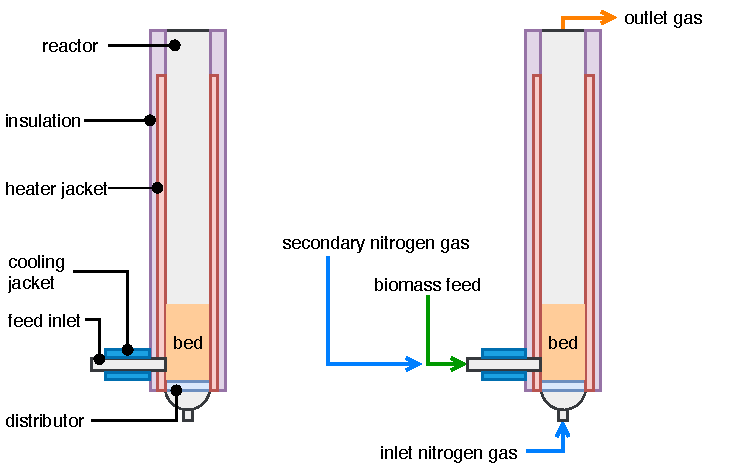
\includegraphics[width=0.8\textwidth]{pyrolyzer-components.pdf}
    \caption{Components (left) and inlet/outlet flows (right) for the BFB biomass pyrolysis reactor in the NREL 2FBR system.}
    \label{fig:pyrolyzer-components}
\end{figure}

\begin{figure}[H]
    \centering
    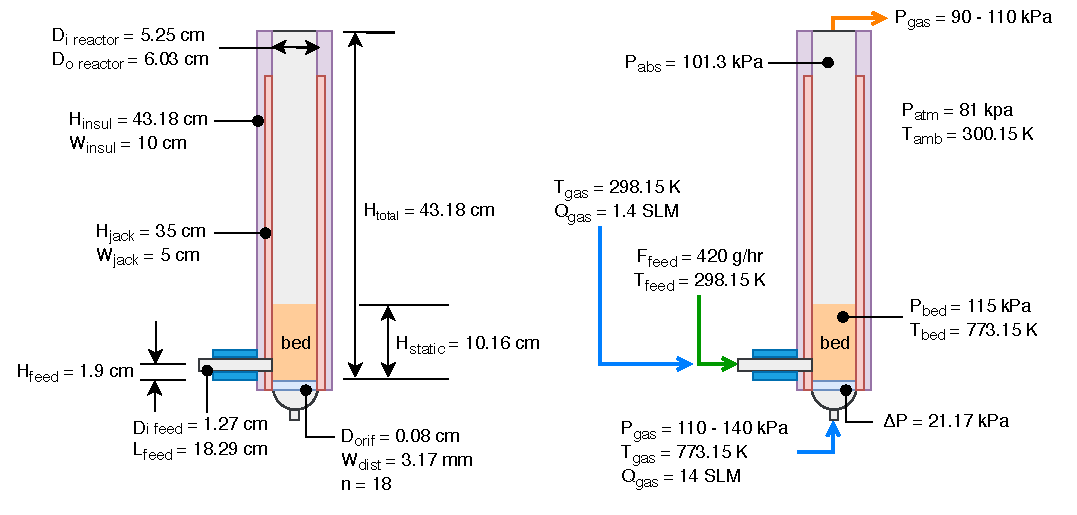
\includegraphics[width=\textwidth]{pyrolyzer-dims-flows.pdf}
    \caption{Dimensions (left) and typical fast pyrolysis operating conditions (right) for the BFB biomass pyrolysis reactor in the NREL 2FBR system.}
    \label{fig:pyrolyzer-dims-flows}
\end{figure}
